% Graphic for TeX using PGF
% Title: /home/gabs48/mit/thesis/graphic/sensors.dia
% Creator: Dia v0.97.2
% CreationDate: Fri Oct 10 15:03:48 2014
% For: gabs48
% \usepackage{tikz}
% The following commands are not supported in PSTricks at present
% We define them conditionally, so when they are implemented,
% this pgf file will use them.
\ifx\du\undefined
  \newlength{\du}
\fi
\setlength{\du}{15\unitlength}
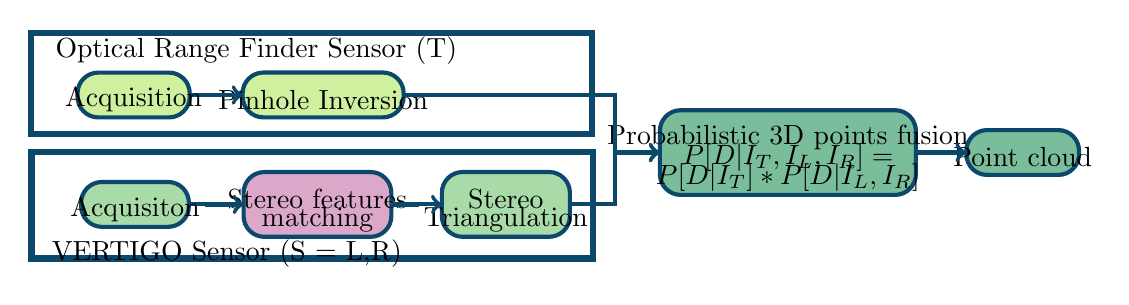
\begin{tikzpicture}
\pgftransformxscale{0.600000}
\pgftransformyscale{-0.600000}
\definecolor{dialinecolor}{rgb}{0.000000, 0.000000, 0.000000}
\pgfsetstrokecolor{dialinecolor}
\definecolor{dialinecolor}{rgb}{1.000000, 1.000000, 1.000000}
\pgfsetfillcolor{dialinecolor}
\pgfsetlinewidth{0.100000\du}
\pgfsetdash{}{0pt}
{\pgfsetcornersarced{\pgfpoint{0.500000\du}{0.500000\du}}\definecolor{dialinecolor}{rgb}{0.811765, 0.941176, 0.619608}
\pgfsetfillcolor{dialinecolor}
\fill (14.962113\du,11.000000\du)--(14.962113\du,12.800000\du)--(21.427113\du,12.800000\du)--(21.427113\du,11.000000\du)--cycle;
}{\pgfsetcornersarced{\pgfpoint{0.500000\du}{0.500000\du}}\definecolor{dialinecolor}{rgb}{0.043137, 0.282353, 0.419608}
\pgfsetstrokecolor{dialinecolor}
\draw (14.962113\du,11.000000\du)--(14.962113\du,12.800000\du)--(21.427113\du,12.800000\du)--(21.427113\du,11.000000\du)--cycle;
}% setfont left to latex
\definecolor{dialinecolor}{rgb}{0.043137, 0.282353, 0.419608}
\pgfsetstrokecolor{dialinecolor}
\node at (18.194613\du,12.095000\du){Pinhole Inversion};
\pgfsetlinewidth{0.100000\du}
\pgfsetdash{}{0pt}
{\pgfsetcornersarced{\pgfpoint{0.500000\du}{0.500000\du}}\definecolor{dialinecolor}{rgb}{0.858824, 0.658824, 0.792157}
\pgfsetfillcolor{dialinecolor}
\fill (15.000000\du,14.995264\du)--(15.000000\du,17.595264\du)--(20.932500\du,17.595264\du)--(20.932500\du,14.995264\du)--cycle;
}{\pgfsetcornersarced{\pgfpoint{0.500000\du}{0.500000\du}}\definecolor{dialinecolor}{rgb}{0.043137, 0.282353, 0.419608}
\pgfsetstrokecolor{dialinecolor}
\draw (15.000000\du,14.995264\du)--(15.000000\du,17.595264\du)--(20.932500\du,17.595264\du)--(20.932500\du,14.995264\du)--cycle;
}% setfont left to latex
\definecolor{dialinecolor}{rgb}{0.043137, 0.282353, 0.419608}
\pgfsetstrokecolor{dialinecolor}
\node at (17.966250\du,16.090264\du){Stereo features};
% setfont left to latex
\definecolor{dialinecolor}{rgb}{0.043137, 0.282353, 0.419608}
\pgfsetstrokecolor{dialinecolor}
\node at (17.966250\du,16.890264\du){ matching};
\pgfsetlinewidth{0.100000\du}
\pgfsetbuttcap
\pgfsetdash{}{0pt}
{
\definecolor{dialinecolor}{rgb}{0.043137, 0.282353, 0.419608}
\pgfsetfillcolor{dialinecolor}
% was here!!!
\pgfsetarrowsend{to}
\definecolor{dialinecolor}{rgb}{0.043137, 0.282353, 0.419608}
\pgfsetstrokecolor{dialinecolor}
\draw (12.837930\du,11.901712\du)--(13.900022\du,11.901712\du)--(13.900022\du,11.900000\du)--(14.962113\du,11.900000\du);
}
% setfont left to latex
\pgfsetlinewidth{0.100000\du}
\pgfsetbuttcap
\pgfsetdash{}{0pt}
{
\definecolor{dialinecolor}{rgb}{0.043137, 0.282353, 0.419608}
\pgfsetfillcolor{dialinecolor}
% was here!!!
\pgfsetarrowsend{to}
\definecolor{dialinecolor}{rgb}{0.043137, 0.282353, 0.419608}
\pgfsetstrokecolor{dialinecolor}
\draw (12.804756\du,16.294325\du)--(13.525000\du,16.294325\du)--(13.525000\du,16.295264\du)--(15.000000\du,16.295264\du);
}
% setfont left to latex
\pgfsetlinewidth{0.100000\du}
\pgfsetdash{}{0pt}
{\pgfsetcornersarced{\pgfpoint{0.500000\du}{0.500000\du}}\definecolor{dialinecolor}{rgb}{0.474510, 0.741176, 0.603922}
\pgfsetfillcolor{dialinecolor}
\fill (31.715151\du,12.511789\du)--(31.715151\du,15.911789\du)--(41.992651\du,15.911789\du)--(41.992651\du,12.511789\du)--cycle;
}{\pgfsetcornersarced{\pgfpoint{0.500000\du}{0.500000\du}}\definecolor{dialinecolor}{rgb}{0.043137, 0.282353, 0.419608}
\pgfsetstrokecolor{dialinecolor}
\draw (31.715151\du,12.511789\du)--(31.715151\du,15.911789\du)--(41.992651\du,15.911789\du)--(41.992651\du,12.511789\du)--cycle;
}% setfont left to latex
\definecolor{dialinecolor}{rgb}{0.043137, 0.282353, 0.419608}
\pgfsetstrokecolor{dialinecolor}
\node at (36.853901\du,13.606789\du){Probabilistic 3D points fusion};
% setfont left to latex
\definecolor{dialinecolor}{rgb}{0.043137, 0.282353, 0.419608}
\pgfsetstrokecolor{dialinecolor}
\node at (36.853901\du,14.406789\du){$P[D|I_T, I_L, I_R] =$};
% setfont left to latex
\definecolor{dialinecolor}{rgb}{0.043137, 0.282353, 0.419608}
\pgfsetstrokecolor{dialinecolor}
\node at (36.853901\du,15.206789\du){$P[D|I_T] * P[D|I_L,I_R]$};
\pgfsetlinewidth{0.100000\du}
\pgfsetdash{}{0pt}
{\pgfsetcornersarced{\pgfpoint{0.500000\du}{0.500000\du}}\definecolor{dialinecolor}{rgb}{0.658824, 0.858824, 0.658824}
\pgfsetfillcolor{dialinecolor}
\fill (22.961654\du,14.994000\du)--(22.961654\du,17.594000\du)--(28.101654\du,17.594000\du)--(28.101654\du,14.994000\du)--cycle;
}{\pgfsetcornersarced{\pgfpoint{0.500000\du}{0.500000\du}}\definecolor{dialinecolor}{rgb}{0.043137, 0.282353, 0.419608}
\pgfsetstrokecolor{dialinecolor}
\draw (22.961654\du,14.994000\du)--(22.961654\du,17.594000\du)--(28.101654\du,17.594000\du)--(28.101654\du,14.994000\du)--cycle;
}% setfont left to latex
\definecolor{dialinecolor}{rgb}{0.043137, 0.282353, 0.419608}
\pgfsetstrokecolor{dialinecolor}
\node at (25.531654\du,16.089000\du){Stereo};
% setfont left to latex
\definecolor{dialinecolor}{rgb}{0.043137, 0.282353, 0.419608}
\pgfsetstrokecolor{dialinecolor}
\node at (25.531654\du,16.889000\du){Triangulation};
\pgfsetlinewidth{0.100000\du}
\pgfsetdash{}{0pt}
{\pgfsetcornersarced{\pgfpoint{0.500000\du}{0.500000\du}}\definecolor{dialinecolor}{rgb}{0.811765, 0.941176, 0.619608}
\pgfsetfillcolor{dialinecolor}
\fill (8.332930\du,11.001712\du)--(8.332930\du,12.801712\du)--(12.837930\du,12.801712\du)--(12.837930\du,11.001712\du)--cycle;
}{\pgfsetcornersarced{\pgfpoint{0.500000\du}{0.500000\du}}\definecolor{dialinecolor}{rgb}{0.043137, 0.282353, 0.419608}
\pgfsetstrokecolor{dialinecolor}
\draw (8.332930\du,11.001712\du)--(8.332930\du,12.801712\du)--(12.837930\du,12.801712\du)--(12.837930\du,11.001712\du)--cycle;
}% setfont left to latex
\definecolor{dialinecolor}{rgb}{0.043137, 0.282353, 0.419608}
\pgfsetstrokecolor{dialinecolor}
\node at (10.585430\du,12.096712\du){Acquisition};
\pgfsetlinewidth{0.100000\du}
\pgfsetdash{}{0pt}
{\pgfsetcornersarced{\pgfpoint{0.500000\du}{0.500000\du}}\definecolor{dialinecolor}{rgb}{0.658824, 0.858824, 0.658824}
\pgfsetfillcolor{dialinecolor}
\fill (8.477256\du,15.394325\du)--(8.477256\du,17.194325\du)--(12.804756\du,17.194325\du)--(12.804756\du,15.394325\du)--cycle;
}{\pgfsetcornersarced{\pgfpoint{0.500000\du}{0.500000\du}}\definecolor{dialinecolor}{rgb}{0.043137, 0.282353, 0.419608}
\pgfsetstrokecolor{dialinecolor}
\draw (8.477256\du,15.394325\du)--(8.477256\du,17.194325\du)--(12.804756\du,17.194325\du)--(12.804756\du,15.394325\du)--cycle;
}% setfont left to latex
\definecolor{dialinecolor}{rgb}{0.043137, 0.282353, 0.419608}
\pgfsetstrokecolor{dialinecolor}
\node at (10.641006\du,16.489325\du){Acquisiton};
\pgfsetlinewidth{0.100000\du}
\pgfsetdash{}{0pt}
{\pgfsetcornersarced{\pgfpoint{0.500000\du}{0.500000\du}}\definecolor{dialinecolor}{rgb}{0.474510, 0.741176, 0.603922}
\pgfsetfillcolor{dialinecolor}
\fill (44.018906\du,13.310344\du)--(44.018906\du,15.110344\du)--(48.543906\du,15.110344\du)--(48.543906\du,13.310344\du)--cycle;
}{\pgfsetcornersarced{\pgfpoint{0.500000\du}{0.500000\du}}\definecolor{dialinecolor}{rgb}{0.043137, 0.282353, 0.419608}
\pgfsetstrokecolor{dialinecolor}
\draw (44.018906\du,13.310344\du)--(44.018906\du,15.110344\du)--(48.543906\du,15.110344\du)--(48.543906\du,13.310344\du)--cycle;
}% setfont left to latex
\definecolor{dialinecolor}{rgb}{0.043137, 0.282353, 0.419608}
\pgfsetstrokecolor{dialinecolor}
\node at (46.281406\du,14.405344\du){Point cloud};
\pgfsetlinewidth{0.100000\du}
\pgfsetbuttcap
\pgfsetdash{}{0pt}
{
\definecolor{dialinecolor}{rgb}{0.043137, 0.282353, 0.419608}
\pgfsetfillcolor{dialinecolor}
% was here!!!
\pgfsetarrowsend{to}
\definecolor{dialinecolor}{rgb}{0.043137, 0.282353, 0.419608}
\pgfsetstrokecolor{dialinecolor}
\draw (20.932500\du,16.295264\du)--(21.947077\du,16.295264\du)--(21.947077\du,16.294000\du)--(22.961654\du,16.294000\du);
}
% setfont left to latex
\pgfsetlinewidth{0.150000\du}
\pgfsetdash{}{0pt}
\pgfsetdash{}{0pt}
\pgfsetmiterjoin
\definecolor{dialinecolor}{rgb}{0.043137, 0.282353, 0.419608}
\pgfsetstrokecolor{dialinecolor}
\draw (6.456786\du,9.414155\du)--(6.456786\du,13.468052\du)--(28.999486\du,13.468052\du)--(28.999486\du,9.414155\du)--cycle;
\pgfsetlinewidth{0.150000\du}
\pgfsetdash{}{0pt}
\pgfsetdash{}{0pt}
\pgfsetmiterjoin
\definecolor{dialinecolor}{rgb}{0.043137, 0.282353, 0.419608}
\pgfsetstrokecolor{dialinecolor}
\draw (6.482533\du,14.183341\du)--(6.482533\du,18.469122\du)--(29.025233\du,18.469122\du)--(29.025233\du,14.183341\du)--cycle;
\pgfsetlinewidth{0.100000\du}
\pgfsetbuttcap
\pgfsetdash{}{0pt}
{
\definecolor{dialinecolor}{rgb}{0.043137, 0.282353, 0.419608}
\pgfsetfillcolor{dialinecolor}
% was here!!!
\pgfsetarrowsend{to}
\definecolor{dialinecolor}{rgb}{0.043137, 0.282353, 0.419608}
\pgfsetstrokecolor{dialinecolor}
\draw (21.412906\du,11.900000\du)--(29.904036\du,11.900000\du)--(29.904036\du,14.211789\du)--(31.700944\du,14.211789\du);
}
% setfont left to latex
\pgfsetlinewidth{0.100000\du}
\pgfsetbuttcap
\pgfsetdash{}{0pt}
{
\definecolor{dialinecolor}{rgb}{0.043137, 0.282353, 0.419608}
\pgfsetfillcolor{dialinecolor}
% was here!!!
\pgfsetarrowsend{to}
\definecolor{dialinecolor}{rgb}{0.043137, 0.282353, 0.419608}
\pgfsetstrokecolor{dialinecolor}
\draw (28.101654\du,16.294000\du)--(29.908403\du,16.294000\du)--(29.908403\du,14.211789\du)--(31.715151\du,14.211789\du);
}
% setfont left to latex
% setfont left to latex
\definecolor{dialinecolor}{rgb}{0.043137, 0.282353, 0.419608}
\pgfsetstrokecolor{dialinecolor}
\node[anchor=west] at (17.728136\du,11.441104\du){};
% setfont left to latex
\definecolor{dialinecolor}{rgb}{0.043137, 0.282353, 0.419608}
\pgfsetstrokecolor{dialinecolor}
\node[anchor=west] at (6.996674\du,10.124534\du){Optical Range Finder Sensor (T)};
% setfont left to latex
\definecolor{dialinecolor}{rgb}{0.043137, 0.282353, 0.419608}
\pgfsetstrokecolor{dialinecolor}
\node[anchor=west] at (6.845126\du,18.270216\du){VERTIGO Sensor (S = L,R)};
\pgfsetlinewidth{0.100000\du}
\pgfsetbuttcap
\pgfsetdash{}{0pt}
{
\definecolor{dialinecolor}{rgb}{0.043137, 0.282353, 0.419608}
\pgfsetfillcolor{dialinecolor}
% was here!!!
\pgfsetarrowsend{to}
\definecolor{dialinecolor}{rgb}{0.043137, 0.282353, 0.419608}
\pgfsetstrokecolor{dialinecolor}
\draw (41.992651\du,14.211789\du)--(43.005779\du,14.211789\du)--(43.005779\du,14.210344\du)--(44.018906\du,14.210344\du);
}
% setfont left to latex
\end{tikzpicture}
